\documentclass[11pt]{article}
\bibliographystyle{unsrtnat}
\usepackage{tabularx} 
\usepackage{subcaption}
\usepackage{caption}
\usepackage{url}
\usepackage{graphicx}
\usepackage{multirow}
\usepackage{amsmath} 
\usepackage{physics}
\usepackage{bm}
\newcommand{\uvec}[1]{\boldsymbol{\hat{\textbf{#1}}}}
\usepackage{graphicx}
\usepackage[margin=1in,letterpaper]{geometry} 
\usepackage[final]{hyperref}
\hypersetup{
	colorlinks=true,
	linkcolor=blue,
	citecolor=black,
	filecolor=magenta,
	urlcolor=blue         
}
\begin{document}
\title{\textbf{\Huge Solar winds}}
\author{Erlend Syljuåsen}
\date{Norwegian University of Science and Technology\\spring 2022}
\maketitle

\section{Theory}
A pure dipole centered at the origin produces a magnetic field given by
$$\vectorbold{B}(\vectorbold{r}) = \frac{\mu_0}{4\pi} \left(\frac{3\vectorbold{r}(\vectorbold{m} \cdot \vectorbold{r})}{r^5} - \frac{\vectorbold{m}}{r^3}\right)$$
The equation of motion, given by the Lorentz force where $\vectorbold{E} = 0$ is 
$$\ddot{\vectorbold{r}} = \frac{q}{m} \dot{\vectorbold{r}} \times \vectorbold{B}$$
Introducing dimensionless variables $\tilde{\vectorbold{r}}= \frac{\vectorbold{r}}{r_0}$, $\tilde{\vectorbold{m}} = \frac{\vectorbold{m}}{m_0}$, $\tilde{t}= \frac{t}{t_0}$, the equation of motion can be rewritten to
\begin{equation}
    \frac{d^2 \tilde{\vectorbold{r}}}{{d\tilde{t}}^2} = \frac{d\tilde{\vectorbold{r}}}{d\tilde{t}} \times \tilde{\vectorbold{B}}
    \label{eq:diff}
\end{equation}
where $$\tilde{\vectorbold{B}} = C\frac{3 \hat{\tilde{\vectorbold{r}}} (\tilde{\vectorbold{m}} \cdot \hat{\tilde{\vectorbold{r}}}) - \tilde{\vectorbold{m}}}{{\tilde{r}}^3}$$ 
and $$ C = \frac{q_{proton}\mu_0 m_0}{m_{proton} 4 \pi v_0 {r_0}^2}$$
The constant C has been chosen such that $\frac{d\tilde{\vectorbold{r}}}{d\tilde{t}}|_{\tilde{t}=0}= v_0$. All the other constants used are displayed in the table below.
\begin{center}
\begin{tabular}{|c|c|c|c|c|c|c|}
\hline
    constant & value & dimension\\
\hline
    $r_0$ & $6371 \cdot 10^3$ & m\\ 
    $m_0$ & $8.22 \cdot 10^{22}$ & Am$^2$\\ 
    $v_0$ & $2.5 \cdot 10^{5}$ & ms$^{-1}$\\
    $q_{proton}$ & $1.6 \cdot 10^{-19}$ & C\\
    $m_{proton}$ & $1.67 \cdot 10^{-27}$ & kg\\
\hline
\end{tabular}
\label{table:constants}
\end{center}

\section{Implementation}
By rewriting \eqref{eq:diff} we obtain two first order differential equations
\begin{equation}
    \frac{d\tilde{\vectorbold{r}}}{d\tilde{t}} = \tilde{\vectorbold{v}}\\
    \hspace{10mm} \frac{d\tilde{\vectorbold{v}}}{d\tilde{t}} = \tilde{\vectorbold{v}} \times \tilde{\vectorbold{B}} 
\end{equation}
In the implementation $\vectorbold{\Lambda}$ is the solution matrix which contains both $\tilde{\vectorbold{v}}$ and $\tilde{\vectorbold{r}}$ for all timesteps. The ODE can then be written as $$\frac{d}{d\tilde{t}} [\tilde{\vectorbold{r}}, \tilde{\vectorbold{v}}]^T = \frac{d\vectorbold{\Lambda}}{d\tilde{t}} = f(\vectorbold{\Lambda}) = [\tilde{\vectorbold{v}}, \tilde{\vectorbold{v}} \times \tilde{\vectorbold{B}}]^{T}$$
RK4 has been chosen as a suitable ODE solver. All code can be found at github \cite{erlensy_github}.

\section{Results}
In figure \ref{fig:mag_field} the magnetic field of the earth has been visualized in two different planes.
\begin{figure}[htp]
    \centering
    \captionsetup{justification=centering}
    \subcaptionbox{xz-plane}{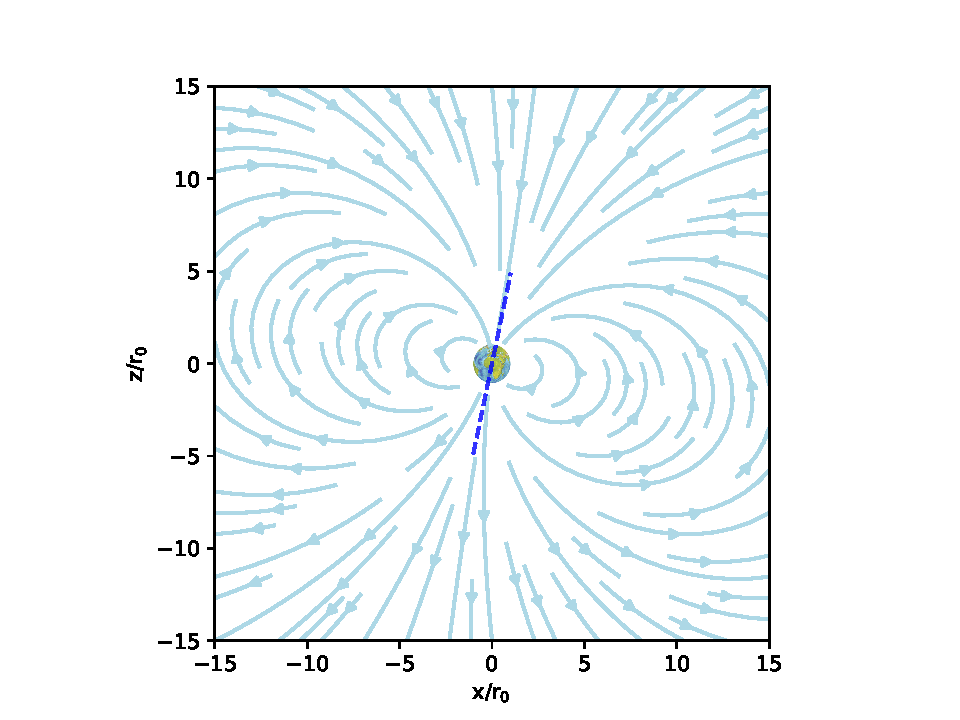
\includegraphics[width=0.44\textwidth]{../figures/magFieldXZ}}
    \hspace{1em}
    \subcaptionbox{xy-plane}{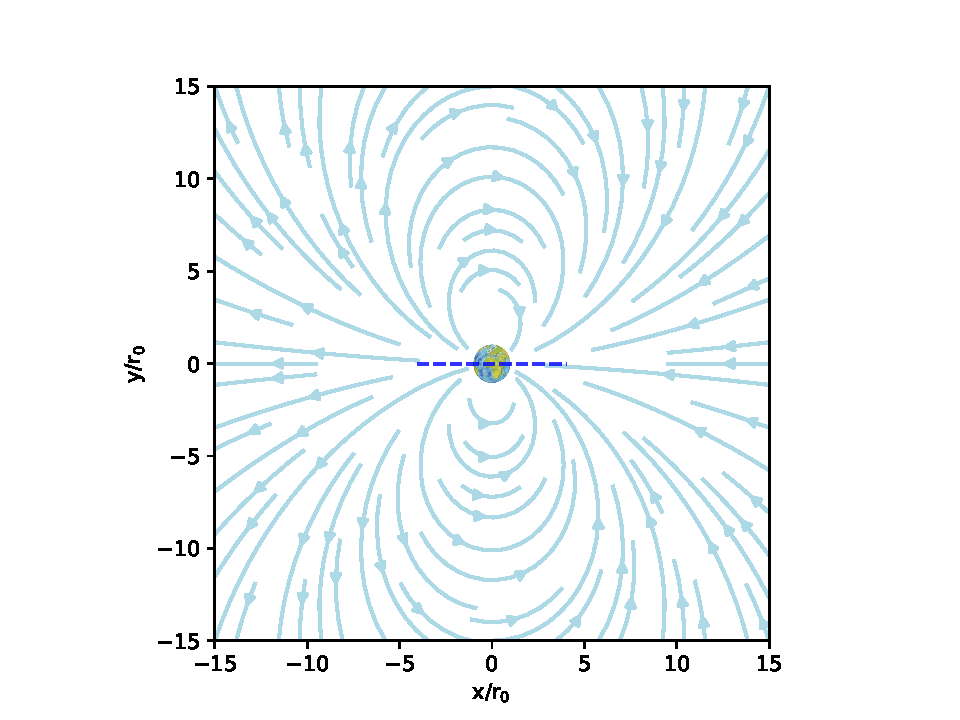
\includegraphics[width=0.44\textwidth]{../figures/magFieldXY}}
    \caption{Magnetic field produced by earth.\\The blue striped line represents the direction of \\earths magnetic moment (the length is scaled).}
    \label{fig:mag_field}
\end{figure}

\begin{thebibliography}{99}
    \bibitem{erlensy_github} Syljuåsen, solar\_winds, \\\url{https://github.com/erlensy/solar_wind}
\end{thebibliography}
\end{document}
